% 5장 주 결과. 0013 · 0014 · 0019 · 0017

\section{주 결과 --- 얼마나 줄었나}

\subsection{지정 직후 거래량}

2020년 6월 23일 지정 직후 3개월 거래량은 \textbf{반사실 대비 $-71 \sim -80\%$}다.
단일 숫자가 아니라 구간으로 적는 이유는 둘이다. 기준 분기를 $-1$, $-3$, $-4$,
$-5$, $-6$ 중 어디에 두어도 $-73 \sim -80\%$ 안에 들어가고(4.5절), 합성대조군이라는
전혀 다른 방법으로 재면 $-71.0\%$다(9.2절).

\textbf{모든 수치는 반사실 대비임을 다시 밝힌다}(0006). ``거래가 80\% 줄었다''가
아니라 ``지정이 없었을 때보다 80\% 적다''는 뜻이다. 통제동도 같은 기간에 줄었고,
그만큼을 뺀 나머지가 여기 적힌 값이다.

\subsection{사건연구 궤적}

한 숫자로 요약하기 전에 분기별 궤적을 먼저 본다. 사전 구간이 평평한지, 효과가
언제 시작해 어떻게 줄어드는지가 여기서 드러난다.

\begin{figure}[htbp]
  \centering
  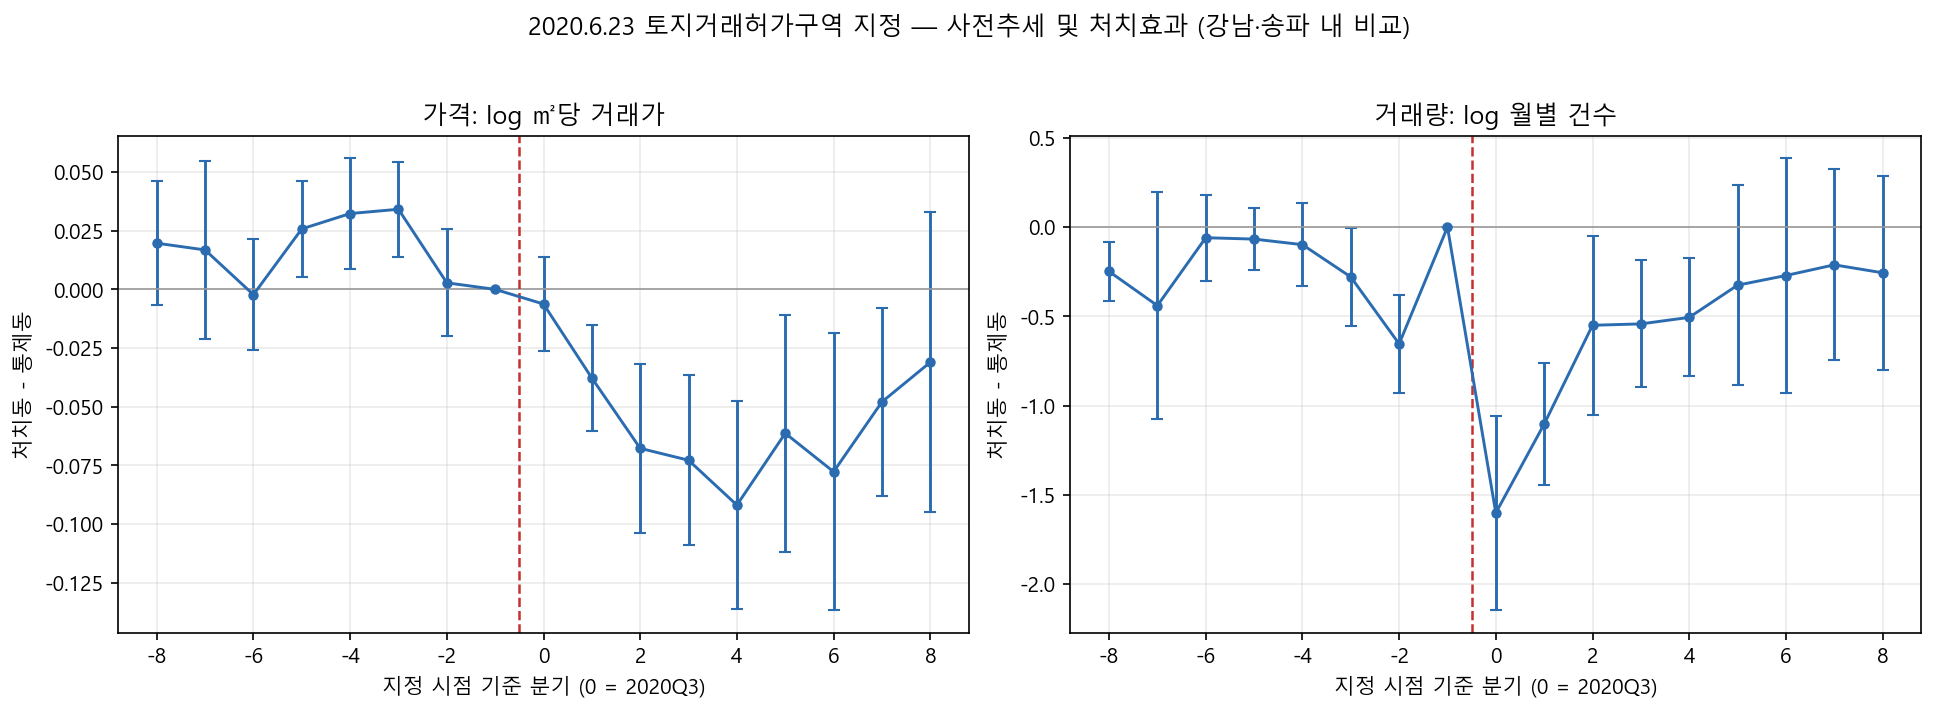
\includegraphics[width=\linewidth]{event_study_2020.png}
  \caption{2020-06-23 지정 사건연구. 왼쪽 가격(log ㎡당가), 오른쪽 거래량
           (log 월별 건수). 세로 점선이 지정 시점, 가로 0선이 기준 분기와
           같다는 뜻이다.}
  \label{fig:event-study-2020}
\end{figure}

그림~\ref{fig:event-study-2020}의 오른쪽이 거래량이다. 지정 분기($k=0$)의 계수가
$-1.6015$이므로 $\exp(-1.6015)-1 = -79.8\%$다. 이후 $k=1$에서 $-66.8\%$,
$k=2$에서 $-42.3\%$, $k=4$에서 $-39.7\%$로 완만해진다.

왼쪽 가격과 대조하면 \textbf{두 결과변수의 모양이 다르다}는 것이 한눈에 보인다.
가격은 사전 구간의 점들이 0 위에 줄줄이 떠 있고 사후에 서서히 내려가며, 거래량은
사전에 0 근처에 모여 있다가 효력일 직후에 수직으로 떨어진다. \textbf{제도가
거래에 마찰을 붙이는 제도라는 사실이 그림에 그대로 나타난다.}

\subsection{적은 클러스터 추론}

처치가 네 개 동뿐이다. 관행적인 군집 표준오차는 묶음이 충분히 많다는 가정 위에
있으므로 \textbf{클러스터가 적으면 표준오차를 작게 잡아 $p$를 과하게 작게
만든다}\citep{mackinnon2017wild}. 실제로 사건연구 $k=0$의 관행 $p$가
$8 \times 10^{-9}$로 나왔다. 그 자체가 증상이다.

두 가지로 다시 쟀다(0019).

\textbf{와일드 클러스터 제약 부트스트랩(WCR).} 귀무가설을 부과한 잔차에 법정동마다
같은 가중을 곱해 가짜 자료를 9,999벌 만들고 $t$ 통계량의 분포를 직접 만든다.
클러스터가 적을 때 권장되는 Webb 6점 분포를 쓴다\citep{webb2014reworking}.

\textbf{무작위화 추론.} 27개 동 가운데 4개를 처치로 고르는 \textbf{모든 경우}
$\binom{27}{4} = 17{,}550$가지를 돌려 진짜 배정이 몇 번째인지 센다
\citep{fisher1935design}. 분포 가정이 전혀 없다.

% 자동 생성 — scripts/build_tables.py. 손으로 고치지 않는다.
% 출처: output/results/06_inference.json
\begin{table}[htbp]
  \centering
  \caption{적은 클러스터 추론. 관행 $p$ 를 버리고 둘을 함께 적는다.}
  \label{tab:inference}
  \begin{tabular}{lrrrr}
    \toprule
    \textbf{사양} & \textbf{효과 (\%)} & \textbf{관행 $p$} & \textbf{WCR $p$} & \textbf{무작위화 순위} \\
    \midrule
    사건연구 k=0 & -79.8 & $<0.001$ & 0.014 & 1 / 17,550 \\
    24개월 이중차분 & -33.5 & 0.016 & 0.050 & 97 / 17,550 \\
    삼중차분 (차이) & -56.1 & 0.002 & 0.027 & 321 / 17,220 \\
    \bottomrule
  \end{tabular}

  \begin{minipage}{\linewidth}\footnotesize
  \textit{주.} 법정동 27개 중 처치가 4개다. WCR 은 Webb 6점 9,999벌, 무작위화는 4개를 고르는 17,550가지 전수.
  \end{minipage}
\end{table}


\begin{figure}[htbp]
  \centering
  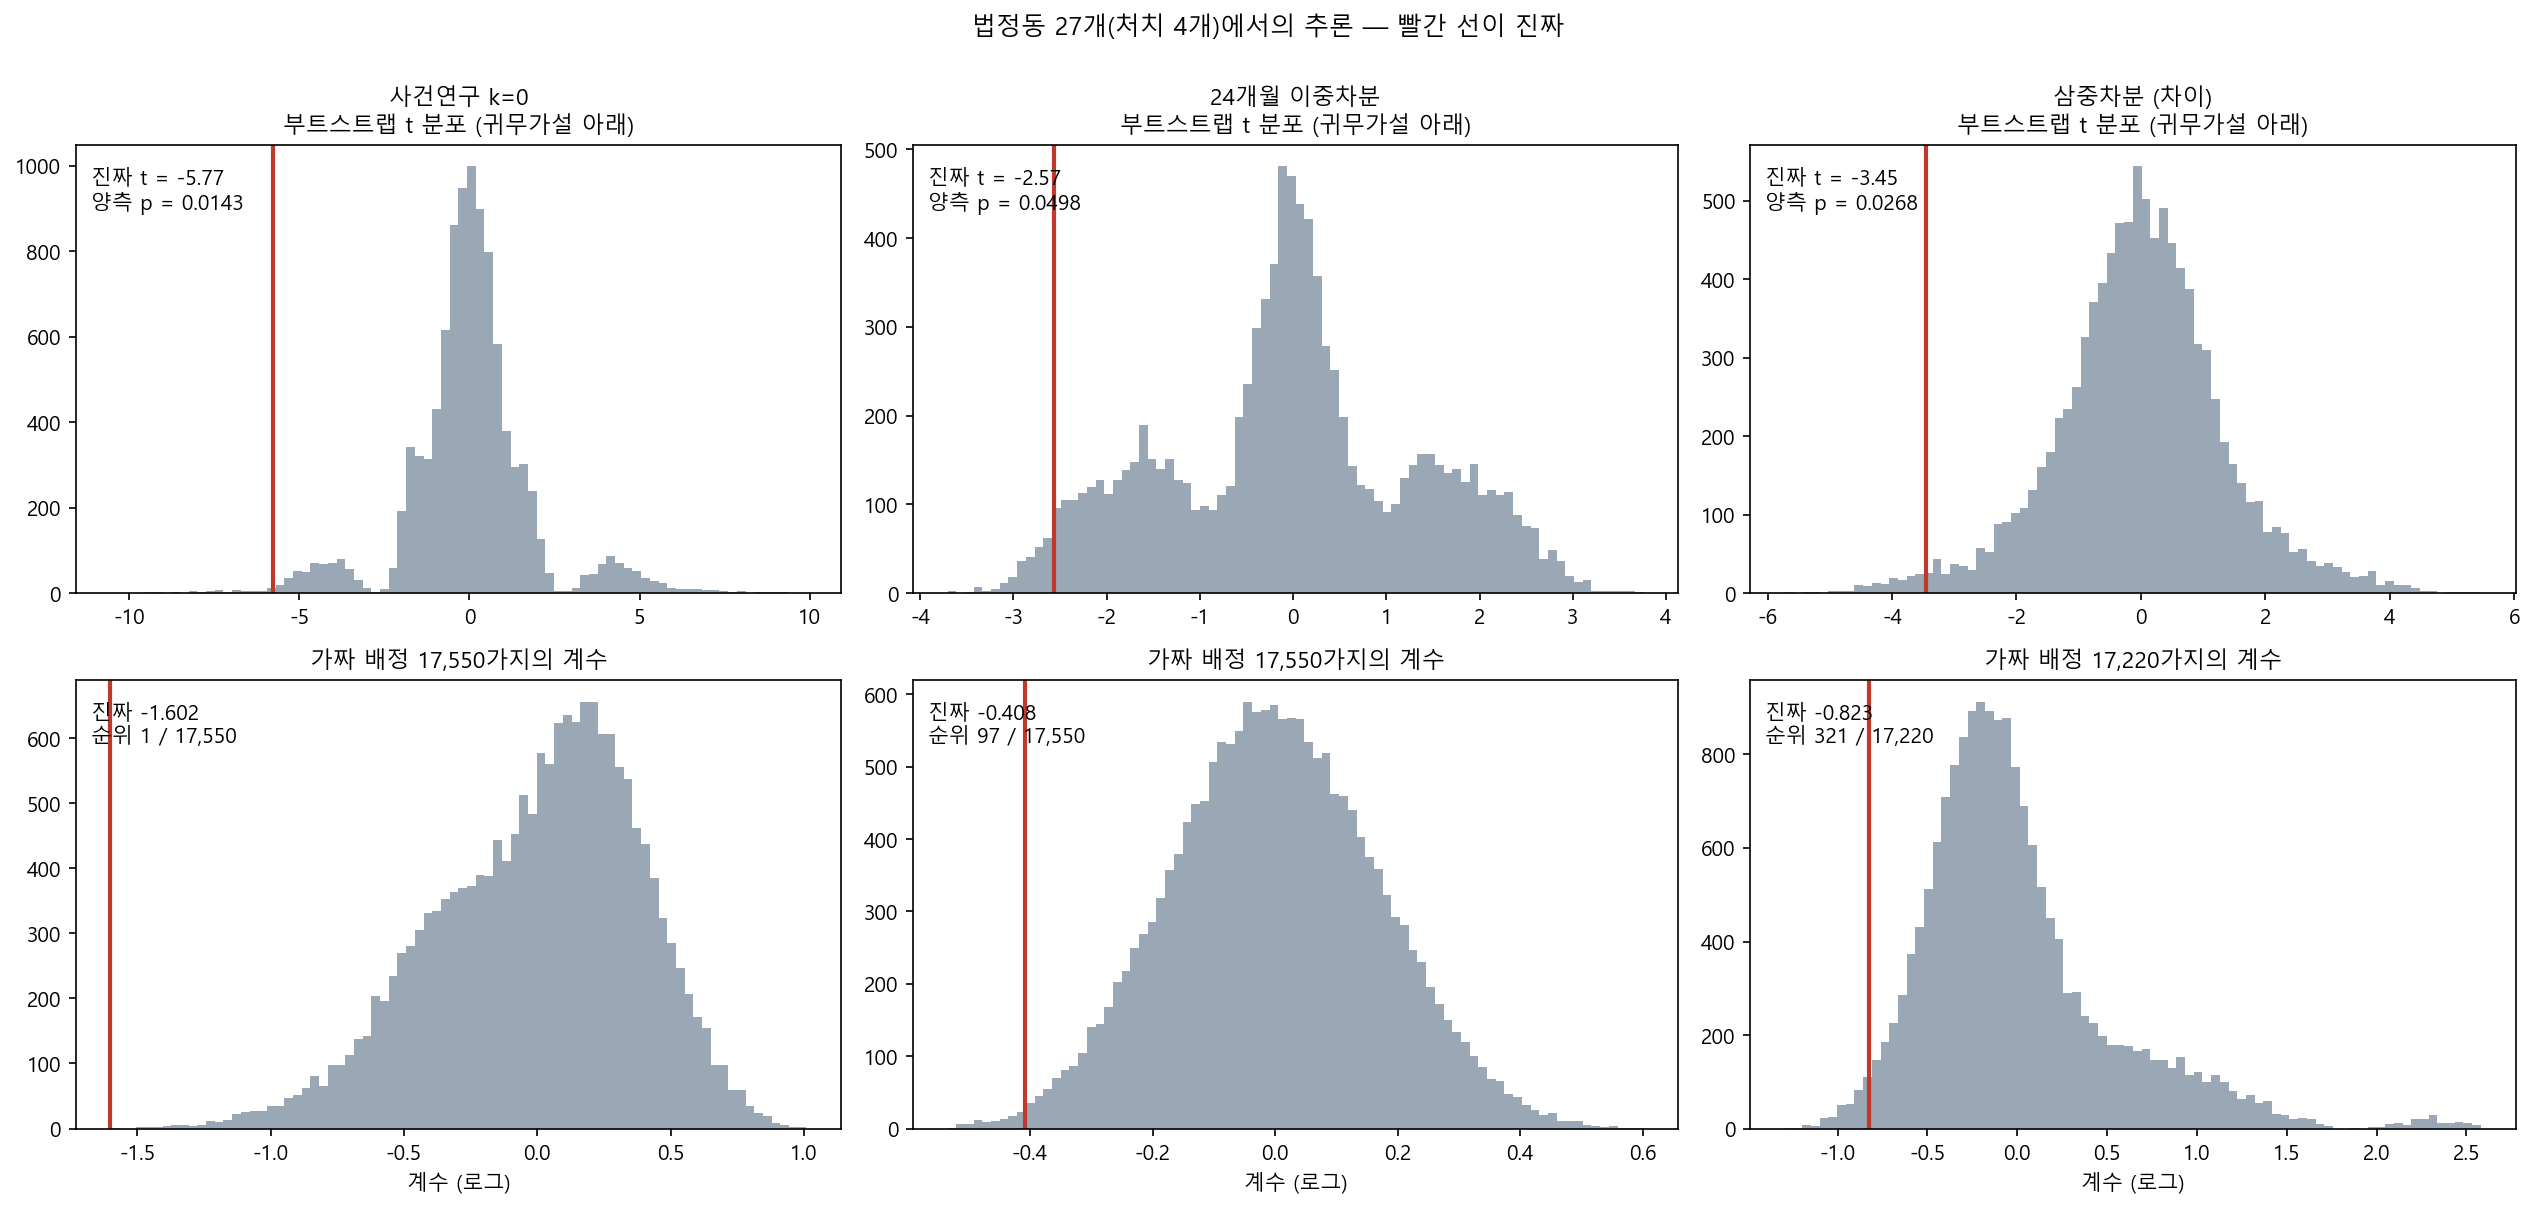
\includegraphics[width=\linewidth]{06_inference.png}
  \caption{와일드 클러스터 부트스트랩과 무작위화 분포. 세로선이 진짜 배정이다.}
  \label{fig:inference}
\end{figure}

\textbf{지정 직후 효과는 어떤 추론으로도 살아남는다.} 17,550가지 배정 중
\textbf{1위}다. 서울 강남·송파의 어느 네 개 동을 골라도 진짜 처치동만큼 지정 직후에
거래가 줄어든 조합은 없다. 관행 $p$ $8\times10^{-9}$는 과장이었지만 결론은 그대로다.

\textbf{다만 ``1위''라는 말은 지정 직후에 한정된다.} 24개월 평균은 97위다.
이 구별을 지키지 않으면 과장이 된다.

\subsection{24개월은 경계에 있다}

사후 24개월을 하나로 묶은 이중차분은 $-33.5\%$이고 WCR $p$가 0.047로
\textbf{0.05에 붙어 있다}. 통제군 오염 동 여섯을 빼면 $-38.4\%$로 커지고 $p$가
0.015로 내려온다(9.3절) --- 경계의 일부는 오염에 의한 감쇠였다.

그러나 \textbf{사전 추세를 모수로 열면 이 값은 버티지 못한다.} 24개월 평균의
붕괴값이 0.05다(8.4절의 방법과 같다). 사전에 관측된 위배의 5\%만 사후에 이어져도
구간이 0을 품는다.

\textbf{그래서 이 보고서는 지속 기간을 말하지 않는다.} 4.5절에서 ``사후
$k \geq 4$는 해석하지 않는다''고 정한 것, 9.2절의 합성대조군에서 사후 27개월
평균이 152개 중 22위($p=0.145$)인 것, 그리고 여기의 붕괴값 0.05가 모두 같은
방향을 가리킨다. \textbf{일시 충격인지 지속적 동결인지는 이 설계로 답할 수 없다.}
